\documentclass{standalone}
\usepackage{tikz}
\usetikzlibrary{patterns, positioning}


\begin{document}
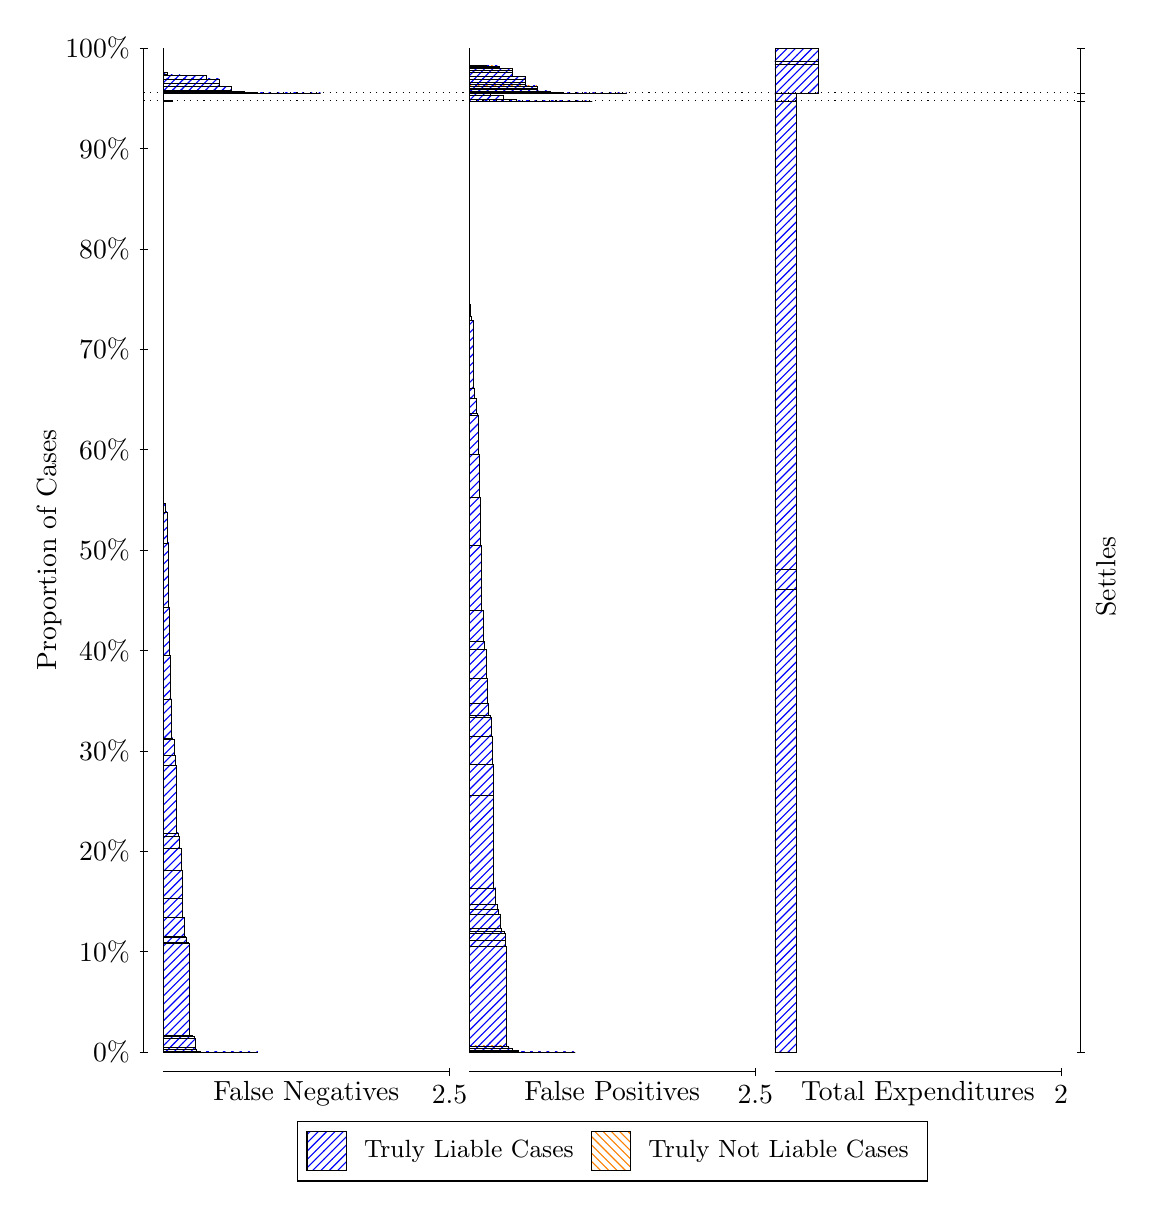
\begin{tikzpicture}
\draw[black, very thin] (1.5,1.75) -- (1.5,14.5);
\node[rotate=90, text=black, anchor=center] at (0.3, 8.125) {Proportion of Cases};
\draw[black, very thin] (1.45,1.75) -- (1.55,1.75);
\node[text=black, anchor=east] at (1.45, 1.75) {0\%};
\draw[black, very thin] (1.45,3.025) -- (1.55,3.025);
\node[text=black, anchor=east] at (1.45, 3.025) {10\%};
\draw[black, very thin] (1.45,4.3) -- (1.55,4.3);
\node[text=black, anchor=east] at (1.45, 4.3) {20\%};
\draw[black, very thin] (1.45,5.575) -- (1.55,5.575);
\node[text=black, anchor=east] at (1.45, 5.575) {30\%};
\draw[black, very thin] (1.45,6.85) -- (1.55,6.85);
\node[text=black, anchor=east] at (1.45, 6.85) {40\%};
\draw[black, very thin] (1.45,8.125) -- (1.55,8.125);
\node[text=black, anchor=east] at (1.45, 8.125) {50\%};
\draw[black, very thin] (1.45,9.4) -- (1.55,9.4);
\node[text=black, anchor=east] at (1.45, 9.4) {60\%};
\draw[black, very thin] (1.45,10.675) -- (1.55,10.675);
\node[text=black, anchor=east] at (1.45, 10.675) {70\%};
\draw[black, very thin] (1.45,11.95) -- (1.55,11.95);
\node[text=black, anchor=east] at (1.45, 11.95) {80\%};
\draw[black, very thin] (1.45,13.225) -- (1.55,13.225);
\node[text=black, anchor=east] at (1.45, 13.225) {90\%};
\draw[black, very thin] (1.45,14.5) -- (1.55,14.5);
\node[text=black, anchor=east] at (1.45, 14.5) {100\%};

\draw[black, very thin] (13.4,1.75) -- (13.4,14.5);
\draw[black, very thin] (13.35,1.75) -- (13.45,1.75);
\node[anchor=west] at (13.35, 1.75) {};
\draw[black, very thin] (13.35,13.828) -- (13.45,13.828);
\node[anchor=west] at (13.35, 13.828) {};
\draw[black, very thin] (13.35,13.931) -- (13.45,13.931);
\node[anchor=west] at (13.35, 13.931) {};
\draw[black, very thin] (13.35,14.5) -- (13.45,14.5);
\node[anchor=west] at (13.35, 14.5) {};

\draw[black, very thin, pattern color=blue, pattern=north east lines] (1.75,1.75) rectangle (2.949,1.75);
\draw[black, very thin, pattern color=blue, pattern=north east lines] (1.75,1.75) rectangle (2.8037,1.75);
\draw[black, very thin, pattern color=blue, pattern=north east lines] (1.75,1.75) rectangle (2.7875,1.75);
\draw[black, very thin, pattern color=blue, pattern=north east lines] (1.75,1.75) rectangle (2.6583,1.75);
\draw[black, very thin, pattern color=blue, pattern=north east lines] (1.75,1.75) rectangle (2.6422,1.75);
\draw[black, very thin, pattern color=blue, pattern=north east lines] (1.75,1.75) rectangle (2.626,1.75);
\draw[black, very thin, pattern color=blue, pattern=north east lines] (1.75,1.75) rectangle (2.5857,1.75);
\draw[black, very thin, pattern color=blue, pattern=north east lines] (1.75,1.75) rectangle (2.513,1.75);
\draw[black, very thin, pattern color=blue, pattern=north east lines] (1.75,1.75) rectangle (2.4969,1.75);
\draw[black, very thin, pattern color=blue, pattern=north east lines] (1.75,1.75) rectangle (2.4807,1.75);
\draw[black, very thin, pattern color=blue, pattern=north east lines] (1.75,1.75) rectangle (2.4646,1.75);
\draw[black, very thin, pattern color=blue, pattern=north east lines] (1.75,1.75) rectangle (2.4403,1.75);
\draw[black, very thin, pattern color=blue, pattern=north east lines] (1.75,1.75) rectangle (2.4242,1.75);
\draw[black, very thin, pattern color=blue, pattern=north east lines] (1.75,1.75) rectangle (2.3677,1.7504);
\draw[black, very thin, pattern color=blue, pattern=north east lines] (1.75,1.7504) rectangle (2.3515,1.7504);
\draw[black, very thin, pattern color=blue, pattern=north east lines] (1.75,1.7504) rectangle (2.3354,1.751);
\draw[black, very thin, pattern color=blue, pattern=north east lines] (1.75,1.751) rectangle (2.3192,1.7515);
\draw[black, very thin, pattern color=blue, pattern=north east lines] (1.75,1.7515) rectangle (2.3031,1.752);
\draw[black, very thin, pattern color=blue, pattern=north east lines] (1.75,1.752) rectangle (2.2789,1.7523);
\draw[black, very thin, pattern color=blue, pattern=north east lines] (1.75,1.7523) rectangle (2.2627,1.7524);
\draw[black, very thin, pattern color=blue, pattern=north east lines] (1.75,1.7524) rectangle (2.2223,1.7528);
\draw[black, very thin, pattern color=blue, pattern=north east lines] (1.75,1.7528) rectangle (2.2062,1.761);
\draw[black, very thin, pattern color=blue, pattern=north east lines] (1.75,1.761) rectangle (2.19,1.7613);
\draw[black, very thin, pattern color=blue, pattern=north east lines] (1.75,1.7613) rectangle (2.1739,1.7869);
\draw[black, very thin, pattern color=blue, pattern=north east lines] (1.75,1.7869) rectangle (2.1577,1.8127);
\draw[black, very thin, pattern color=blue, pattern=north east lines] (1.75,1.8127) rectangle (2.1497,1.9212);
\draw[black, very thin, pattern color=blue, pattern=north east lines] (1.75,1.9212) rectangle (2.1416,1.9475);
\draw[black, very thin, pattern color=blue, pattern=north east lines] (1.75,1.9475) rectangle (2.1174,1.962);
\draw[black, very thin, pattern color=blue, pattern=north east lines] (1.75,1.962) rectangle (2.1012,1.9653);
\draw[black, very thin, pattern color=blue, pattern=north east lines] (1.75,1.9653) rectangle (2.077,3.126);
\draw[black, very thin, pattern color=blue, pattern=north east lines] (1.75,3.126) rectangle (2.0609,3.1393);
\draw[black, very thin, pattern color=blue, pattern=north east lines] (1.75,3.1393) rectangle (2.0447,3.2096);
\draw[black, very thin, pattern color=blue, pattern=north east lines] (1.75,3.2096) rectangle (2.0286,3.2137);
\draw[black, very thin, pattern color=blue, pattern=north east lines] (1.75,3.2137) rectangle (2.0124,3.4545);
\draw[black, very thin, pattern color=blue, pattern=north east lines] (1.75,3.4545) rectangle (1.9963,3.7002);
\draw[black, very thin, pattern color=blue, pattern=north east lines] (1.75,3.7002) rectangle (1.9882,4.0591);
\draw[black, very thin, pattern color=blue, pattern=north east lines] (1.75,4.0591) rectangle (1.9801,4.3309);
\draw[black, very thin, pattern color=blue, pattern=north east lines] (1.75,4.3309) rectangle (1.9559,4.4906);
\draw[black, very thin, pattern color=blue, pattern=north east lines] (1.75,4.4906) rectangle (1.9397,4.5325);
\draw[black, very thin, pattern color=blue, pattern=north east lines] (1.75,4.5325) rectangle (1.9155,5.3947);
\draw[black, very thin, pattern color=blue, pattern=north east lines] (1.75,5.3947) rectangle (1.8994,5.521);
\draw[black, very thin, pattern color=blue, pattern=north east lines] (1.75,5.521) rectangle (1.8832,5.7211);
\draw[black, very thin, pattern color=blue, pattern=north east lines] (1.75,5.7211) rectangle (1.8671,5.7381);
\draw[black, very thin, pattern color=blue, pattern=north east lines] (1.75,5.7381) rectangle (1.8509,6.2356);
\draw[black, very thin, pattern color=blue, pattern=north east lines] (1.75,6.2356) rectangle (1.8348,6.7864);
\draw[black, very thin, pattern color=blue, pattern=north east lines] (1.75,6.7864) rectangle (1.8267,7.3961);
\draw[black, very thin, pattern color=blue, pattern=north east lines] (1.75,7.3961) rectangle (1.8186,8.2162);
\draw[black, very thin, pattern color=blue, pattern=north east lines] (1.75,8.2162) rectangle (1.7944,8.6078);
\draw[black, very thin, pattern color=blue, pattern=north east lines] (1.75,8.6078) rectangle (1.7783,8.7136);
\draw[black, very thin, pattern color=blue, pattern=north east lines] (1.75,8.7136) rectangle (1.754,9.083);
\draw[black, very thin, pattern color=orange, pattern=north west lines] (1.75,9.083) rectangle (1.75,9.083);
\draw[black, very thin, pattern color=blue, pattern=north east lines] (1.75,9.083) rectangle (1.75,13.828);
\draw[black, very thin, pattern color=blue, pattern=north east lines] (1.75,13.828) rectangle (1.859,13.832);
\draw[black, very thin, pattern color=orange, pattern=north west lines] (1.75,13.832) rectangle (1.75,13.832);
\draw[black, very thin, pattern color=blue, pattern=north east lines] (1.75,13.832) rectangle (1.75,13.931);
\draw[black, very thin, pattern color=blue, pattern=north east lines] (1.75,13.931) rectangle (3.7483,13.931);
\draw[black, very thin, pattern color=blue, pattern=north east lines] (1.75,13.931) rectangle (3.5869,13.931);
\draw[black, very thin, pattern color=blue, pattern=north east lines] (1.75,13.931) rectangle (3.4254,13.931);
\draw[black, very thin, pattern color=blue, pattern=north east lines] (1.75,13.931) rectangle (3.2639,13.931);
\draw[black, very thin, pattern color=blue, pattern=north east lines] (1.75,13.931) rectangle (3.2639,13.931);
\draw[black, very thin, pattern color=blue, pattern=north east lines] (1.75,13.931) rectangle (3.1024,13.931);
\draw[black, very thin, pattern color=blue, pattern=north east lines] (1.75,13.931) rectangle (2.9409,13.934);
\draw[black, very thin, pattern color=blue, pattern=north east lines] (1.75,13.934) rectangle (2.7794,13.941);
\draw[black, very thin, pattern color=blue, pattern=north east lines] (1.75,13.941) rectangle (2.7794,13.954);
\draw[black, very thin, pattern color=blue, pattern=north east lines] (1.75,13.954) rectangle (2.618,13.968);
\draw[black, very thin, pattern color=blue, pattern=north east lines] (1.75,13.968) rectangle (2.618,14.015);
\draw[black, very thin, pattern color=blue, pattern=north east lines] (1.75,14.015) rectangle (2.6099,14.015);
\draw[black, very thin, pattern color=blue, pattern=north east lines] (1.75,14.015) rectangle (2.4565,14.048);
\draw[black, very thin, pattern color=blue, pattern=north east lines] (1.75,14.048) rectangle (2.4565,14.101);
\draw[black, very thin, pattern color=blue, pattern=north east lines] (1.75,14.101) rectangle (2.4565,14.107);
\draw[black, very thin, pattern color=blue, pattern=north east lines] (1.75,14.107) rectangle (2.4484,14.107);
\draw[black, very thin, pattern color=blue, pattern=north east lines] (1.75,14.107) rectangle (2.4484,14.107);
\draw[black, very thin, pattern color=blue, pattern=north east lines] (1.75,14.107) rectangle (2.295,14.151);
\draw[black, very thin, pattern color=blue, pattern=north east lines] (1.75,14.151) rectangle (2.2869,14.151);
\draw[black, very thin, pattern color=blue, pattern=north east lines] (1.75,14.151) rectangle (2.1335,14.152);
\draw[black, very thin, pattern color=blue, pattern=north east lines] (1.75,14.152) rectangle (2.1335,14.155);
\draw[black, very thin, pattern color=blue, pattern=north east lines] (1.75,14.155) rectangle (2.1335,14.156);
\draw[black, very thin, pattern color=blue, pattern=north east lines] (1.75,14.156) rectangle (2.1254,14.156);
\draw[black, very thin, pattern color=blue, pattern=north east lines] (1.75,14.156) rectangle (2.1254,14.156);
\draw[black, very thin, pattern color=blue, pattern=north east lines] (1.75,14.156) rectangle (1.972,14.156);
\draw[black, very thin, pattern color=blue, pattern=north east lines] (1.75,14.156) rectangle (1.972,14.156);
\draw[black, very thin, pattern color=blue, pattern=north east lines] (1.75,14.156) rectangle (1.964,14.158);
\draw[black, very thin, pattern color=blue, pattern=north east lines] (1.75,14.158) rectangle (1.8106,14.158);
\draw[black, very thin, pattern color=blue, pattern=north east lines] (1.75,14.158) rectangle (1.8106,14.158);
\draw[black, very thin, pattern color=blue, pattern=north east lines] (1.75,14.158) rectangle (1.8025,14.161);
\draw[black, very thin, pattern color=blue, pattern=north east lines] (1.75,14.161) rectangle (1.8025,14.187);
\draw[black, very thin, pattern color=orange, pattern=north west lines] (1.75,14.187) rectangle (1.75,14.187);
\draw[black, very thin, pattern color=blue, pattern=north east lines] (1.75,14.187) rectangle (1.75,14.5);
\draw[black, very thin, pattern color=orange, pattern=north west lines] (5.6333,1.75) rectangle (6.9777,1.75);
\draw[black, very thin, pattern color=blue, pattern=north east lines] (5.6333,1.75) rectangle (6.9777,1.75);
\draw[black, very thin, pattern color=orange, pattern=north west lines] (5.6333,1.75) rectangle (6.905,1.75);
\draw[black, very thin, pattern color=blue, pattern=north east lines] (5.6333,1.75) rectangle (6.905,1.75);
\draw[black, very thin, pattern color=orange, pattern=north west lines] (5.6333,1.75) rectangle (6.8323,1.75);
\draw[black, very thin, pattern color=blue, pattern=north east lines] (5.6333,1.75) rectangle (6.8323,1.75);
\draw[black, very thin, pattern color=blue, pattern=north east lines] (5.6333,1.75) rectangle (6.8162,1.75);
\draw[black, very thin, pattern color=blue, pattern=north east lines] (5.6333,1.75) rectangle (6.7435,1.75);
\draw[black, very thin, pattern color=orange, pattern=north west lines] (5.6333,1.75) rectangle (6.687,1.75);
\draw[black, very thin, pattern color=blue, pattern=north east lines] (5.6333,1.75) rectangle (6.687,1.75);
\draw[black, very thin, pattern color=blue, pattern=north east lines] (5.6333,1.75) rectangle (6.6709,1.75);
\draw[black, very thin, pattern color=blue, pattern=north east lines] (5.6333,1.75) rectangle (6.6547,1.75);
\draw[black, very thin, pattern color=orange, pattern=north west lines] (5.6333,1.75) rectangle (6.6143,1.75);
\draw[black, very thin, pattern color=blue, pattern=north east lines] (5.6333,1.75) rectangle (6.6143,1.75);
\draw[black, very thin, pattern color=blue, pattern=north east lines] (5.6333,1.75) rectangle (6.582,1.75);
\draw[black, very thin, pattern color=orange, pattern=north west lines] (5.6333,1.75) rectangle (6.5417,1.75);
\draw[black, very thin, pattern color=blue, pattern=north east lines] (5.6333,1.75) rectangle (6.5417,1.75);
\draw[black, very thin, pattern color=blue, pattern=north east lines] (5.6333,1.75) rectangle (6.5255,1.75);
\draw[black, very thin, pattern color=blue, pattern=north east lines] (5.6333,1.75) rectangle (6.5094,1.75);
\draw[black, very thin, pattern color=blue, pattern=north east lines] (5.6333,1.75) rectangle (6.4932,1.75);
\draw[black, very thin, pattern color=orange, pattern=north west lines] (5.6333,1.75) rectangle (6.469,1.75);
\draw[black, very thin, pattern color=blue, pattern=north east lines] (5.6333,1.75) rectangle (6.469,1.75);
\draw[black, very thin, pattern color=blue, pattern=north east lines] (5.6333,1.75) rectangle (6.4529,1.75);
\draw[black, very thin, pattern color=blue, pattern=north east lines] (5.6333,1.75) rectangle (6.4206,1.75);
\draw[black, very thin, pattern color=orange, pattern=north west lines] (5.6333,1.75) rectangle (6.3963,1.75);
\draw[black, very thin, pattern color=blue, pattern=north east lines] (5.6333,1.75) rectangle (6.3963,1.75);
\draw[black, very thin, pattern color=blue, pattern=north east lines] (5.6333,1.75) rectangle (6.3802,1.75);
\draw[black, very thin, pattern color=blue, pattern=north east lines] (5.6333,1.75) rectangle (6.364,1.7501);
\draw[black, very thin, pattern color=blue, pattern=north east lines] (5.6333,1.7501) rectangle (6.3479,1.7506);
\draw[black, very thin, pattern color=blue, pattern=north east lines] (5.6333,1.7506) rectangle (6.3317,1.7506);
\draw[black, very thin, pattern color=blue, pattern=north east lines] (5.6333,1.7506) rectangle (6.3075,1.7509);
\draw[black, very thin, pattern color=blue, pattern=north east lines] (5.6333,1.7509) rectangle (6.2914,1.7514);
\draw[black, very thin, pattern color=blue, pattern=north east lines] (5.6333,1.7514) rectangle (6.2591,1.7548);
\draw[black, very thin, pattern color=orange, pattern=north west lines] (5.6333,1.7548) rectangle (6.251,1.7548);
\draw[black, very thin, pattern color=blue, pattern=north east lines] (5.6333,1.7548) rectangle (6.251,1.7662);
\draw[black, very thin, pattern color=blue, pattern=north east lines] (5.6333,1.7662) rectangle (6.2349,1.7668);
\draw[black, very thin, pattern color=blue, pattern=north east lines] (5.6333,1.7668) rectangle (6.2187,1.767);
\draw[black, very thin, pattern color=blue, pattern=north east lines] (5.6333,1.767) rectangle (6.2026,1.7683);
\draw[black, very thin, pattern color=blue, pattern=north east lines] (5.6333,1.7683) rectangle (6.1864,1.7909);
\draw[black, very thin, pattern color=blue, pattern=north east lines] (5.6333,1.7909) rectangle (6.1703,1.7944);
\draw[black, very thin, pattern color=blue, pattern=north east lines] (5.6333,1.7944) rectangle (6.146,1.8017);
\draw[black, very thin, pattern color=blue, pattern=north east lines] (5.6333,1.8017) rectangle (6.1299,1.8261);
\draw[black, very thin, pattern color=orange, pattern=north west lines] (5.6333,1.8261) rectangle (6.1057,1.8261);
\draw[black, very thin, pattern color=blue, pattern=north east lines] (5.6333,1.8261) rectangle (6.1057,3.0892);
\draw[black, very thin, pattern color=blue, pattern=north east lines] (5.6333,3.0892) rectangle (6.0976,3.1643);
\draw[black, very thin, pattern color=blue, pattern=north east lines] (5.6333,3.1643) rectangle (6.0895,3.2546);
\draw[black, very thin, pattern color=blue, pattern=north east lines] (5.6333,3.2546) rectangle (6.0734,3.2806);
\draw[black, very thin, pattern color=blue, pattern=north east lines] (5.6333,3.2806) rectangle (6.0572,3.2837);
\draw[black, very thin, pattern color=blue, pattern=north east lines] (5.6333,3.2837) rectangle (6.0411,3.3152);
\draw[black, very thin, pattern color=blue, pattern=north east lines] (5.6333,3.3152) rectangle (6.0249,3.5);
\draw[black, very thin, pattern color=blue, pattern=north east lines] (5.6333,3.5) rectangle (6.0088,3.5639);
\draw[black, very thin, pattern color=blue, pattern=north east lines] (5.6333,3.5639) rectangle (5.9846,3.6197);
\draw[black, very thin, pattern color=blue, pattern=north east lines] (5.6333,3.6197) rectangle (5.9684,3.8339);
\draw[black, very thin, pattern color=blue, pattern=north east lines] (5.6333,3.8339) rectangle (5.9442,5.0098);
\draw[black, very thin, pattern color=blue, pattern=north east lines] (5.6333,5.0098) rectangle (5.9361,5.4035);
\draw[black, very thin, pattern color=blue, pattern=north east lines] (5.6333,5.4035) rectangle (5.928,5.7653);
\draw[black, very thin, pattern color=blue, pattern=north east lines] (5.6333,5.7653) rectangle (5.9119,6.0062);
\draw[black, very thin, pattern color=blue, pattern=north east lines] (5.6333,6.0062) rectangle (5.8957,6.0217);
\draw[black, very thin, pattern color=blue, pattern=north east lines] (5.6333,6.0217) rectangle (5.8796,6.1808);
\draw[black, very thin, pattern color=blue, pattern=north east lines] (5.6333,6.1808) rectangle (5.8634,6.4949);
\draw[black, very thin, pattern color=blue, pattern=north east lines] (5.6333,6.4949) rectangle (5.8473,6.8643);
\draw[black, very thin, pattern color=blue, pattern=north east lines] (5.6333,6.8643) rectangle (5.8231,6.9701);
\draw[black, very thin, pattern color=blue, pattern=north east lines] (5.6333,6.9701) rectangle (5.8069,7.3617);
\draw[black, very thin, pattern color=blue, pattern=north east lines] (5.6333,7.3617) rectangle (5.7827,8.1818);
\draw[black, very thin, pattern color=blue, pattern=north east lines] (5.6333,8.1818) rectangle (5.7746,8.7916);
\draw[black, very thin, pattern color=blue, pattern=north east lines] (5.6333,8.7916) rectangle (5.7666,9.3424);
\draw[black, very thin, pattern color=blue, pattern=north east lines] (5.6333,9.3424) rectangle (5.7504,9.8399);
\draw[black, very thin, pattern color=blue, pattern=north east lines] (5.6333,9.8399) rectangle (5.7343,9.8569);
\draw[black, very thin, pattern color=blue, pattern=north east lines] (5.6333,9.8569) rectangle (5.7181,10.057);
\draw[black, very thin, pattern color=blue, pattern=north east lines] (5.6333,10.057) rectangle (5.702,10.183);
\draw[black, very thin, pattern color=blue, pattern=north east lines] (5.6333,10.183) rectangle (5.6858,11.045);
\draw[black, very thin, pattern color=blue, pattern=north east lines] (5.6333,11.045) rectangle (5.6616,11.087);
\draw[black, very thin, pattern color=blue, pattern=north east lines] (5.6333,11.087) rectangle (5.6454,11.247);
\draw[black, very thin, pattern color=blue, pattern=north east lines] (5.6333,11.247) rectangle (5.6333,13.828);
\draw[black, very thin, pattern color=orange, pattern=north west lines] (5.6333,13.828) rectangle (7.1957,13.828);
\draw[black, very thin, pattern color=blue, pattern=north east lines] (5.6333,13.828) rectangle (7.1957,13.828);
\draw[black, very thin, pattern color=blue, pattern=north east lines] (5.6333,13.828) rectangle (7.0342,13.828);
\draw[black, very thin, pattern color=blue, pattern=north east lines] (5.6333,13.828) rectangle (6.8727,13.828);
\draw[black, very thin, pattern color=blue, pattern=north east lines] (5.6333,13.828) rectangle (6.7112,13.828);
\draw[black, very thin, pattern color=blue, pattern=north east lines] (5.6333,13.828) rectangle (6.5497,13.828);
\draw[black, very thin, pattern color=blue, pattern=north east lines] (5.6333,13.828) rectangle (6.3883,13.83);
\draw[black, very thin, pattern color=blue, pattern=north east lines] (5.6333,13.83) rectangle (6.2268,13.851);
\draw[black, very thin, pattern color=blue, pattern=north east lines] (5.6333,13.851) rectangle (6.0653,13.9);
\draw[black, very thin, pattern color=blue, pattern=north east lines] (5.6333,13.9) rectangle (5.9038,13.926);
\draw[black, very thin, pattern color=blue, pattern=north east lines] (5.6333,13.926) rectangle (5.7423,13.931);
\draw[black, very thin, pattern color=orange, pattern=north west lines] (5.6333,13.931) rectangle (7.6317,13.931);
\draw[black, very thin, pattern color=blue, pattern=north east lines] (5.6333,13.931) rectangle (7.6317,13.931);
\draw[black, very thin, pattern color=orange, pattern=north west lines] (5.6333,13.931) rectangle (7.4702,13.931);
\draw[black, very thin, pattern color=blue, pattern=north east lines] (5.6333,13.931) rectangle (7.4702,13.931);
\draw[black, very thin, pattern color=orange, pattern=north west lines] (5.6333,13.931) rectangle (7.3087,13.931);
\draw[black, very thin, pattern color=blue, pattern=north east lines] (5.6333,13.931) rectangle (7.3087,13.931);
\draw[black, very thin, pattern color=blue, pattern=north east lines] (5.6333,13.931) rectangle (7.1472,13.931);
\draw[black, very thin, pattern color=orange, pattern=north west lines] (5.6333,13.931) rectangle (7.1472,13.931);
\draw[black, very thin, pattern color=blue, pattern=north east lines] (5.6333,13.931) rectangle (7.1472,13.931);
\draw[black, very thin, pattern color=orange, pattern=north west lines] (5.6333,13.931) rectangle (6.9857,13.931);
\draw[black, very thin, pattern color=blue, pattern=north east lines] (5.6333,13.931) rectangle (6.9857,13.931);
\draw[black, very thin, pattern color=blue, pattern=north east lines] (5.6333,13.931) rectangle (6.9857,13.931);
\draw[black, very thin, pattern color=blue, pattern=north east lines] (5.6333,13.931) rectangle (6.9857,13.931);
\draw[black, very thin, pattern color=orange, pattern=north west lines] (5.6333,13.931) rectangle (6.8243,13.931);
\draw[black, very thin, pattern color=blue, pattern=north east lines] (5.6333,13.931) rectangle (6.8243,13.935);
\draw[black, very thin, pattern color=blue, pattern=north east lines] (5.6333,13.935) rectangle (6.8243,13.935);
\draw[black, very thin, pattern color=blue, pattern=north east lines] (5.6333,13.935) rectangle (6.6628,13.941);
\draw[black, very thin, pattern color=orange, pattern=north west lines] (5.6333,13.941) rectangle (6.6628,13.941);
\draw[black, very thin, pattern color=blue, pattern=north east lines] (5.6333,13.941) rectangle (6.6628,13.955);
\draw[black, very thin, pattern color=blue, pattern=north east lines] (5.6333,13.955) rectangle (6.5013,13.97);
\draw[black, very thin, pattern color=blue, pattern=north east lines] (5.6333,13.97) rectangle (6.5013,13.99);
\draw[black, very thin, pattern color=blue, pattern=north east lines] (5.6333,13.99) rectangle (6.5013,14.019);
\draw[black, very thin, pattern color=orange, pattern=north west lines] (5.6333,14.019) rectangle (6.4932,14.019);
\draw[black, very thin, pattern color=blue, pattern=north east lines] (5.6333,14.019) rectangle (6.4932,14.019);
\draw[black, very thin, pattern color=blue, pattern=north east lines] (5.6333,14.019) rectangle (6.3398,14.044);
\draw[black, very thin, pattern color=blue, pattern=north east lines] (5.6333,14.044) rectangle (6.3398,14.07);
\draw[black, very thin, pattern color=blue, pattern=north east lines] (5.6333,14.07) rectangle (6.3398,14.109);
\draw[black, very thin, pattern color=blue, pattern=north east lines] (5.6333,14.109) rectangle (6.3398,14.136);
\draw[black, very thin, pattern color=orange, pattern=north west lines] (5.6333,14.136) rectangle (6.3317,14.136);
\draw[black, very thin, pattern color=blue, pattern=north east lines] (5.6333,14.136) rectangle (6.3317,14.136);
\draw[black, very thin, pattern color=blue, pattern=north east lines] (5.6333,14.136) rectangle (6.3317,14.136);
\draw[black, very thin, pattern color=blue, pattern=north east lines] (5.6333,14.136) rectangle (6.1783,14.186);
\draw[black, very thin, pattern color=blue, pattern=north east lines] (5.6333,14.186) rectangle (6.1783,14.218);
\draw[black, very thin, pattern color=blue, pattern=north east lines] (5.6333,14.218) rectangle (6.1783,14.244);
\draw[black, very thin, pattern color=blue, pattern=north east lines] (5.6333,14.244) rectangle (6.1703,14.244);
\draw[black, very thin, pattern color=orange, pattern=north west lines] (5.6333,14.244) rectangle (6.1703,14.244);
\draw[black, very thin, pattern color=blue, pattern=north east lines] (5.6333,14.244) rectangle (6.1703,14.244);
\draw[black, very thin, pattern color=blue, pattern=north east lines] (5.6333,14.244) rectangle (6.0169,14.256);
\draw[black, very thin, pattern color=blue, pattern=north east lines] (5.6333,14.256) rectangle (6.0169,14.272);
\draw[black, very thin, pattern color=blue, pattern=north east lines] (5.6333,14.272) rectangle (6.0169,14.273);
\draw[black, very thin, pattern color=blue, pattern=north east lines] (5.6333,14.273) rectangle (6.0088,14.273);
\draw[black, very thin, pattern color=blue, pattern=north east lines] (5.6333,14.273) rectangle (6.0088,14.273);
\draw[black, very thin, pattern color=orange, pattern=north west lines] (5.6333,14.273) rectangle (6.0088,14.273);
\draw[black, very thin, pattern color=blue, pattern=north east lines] (5.6333,14.273) rectangle (6.0088,14.273);
\draw[black, very thin, pattern color=blue, pattern=north east lines] (5.6333,14.273) rectangle (5.8554,14.274);
\draw[black, very thin, pattern color=blue, pattern=north east lines] (5.6333,14.274) rectangle (5.8554,14.275);
\draw[black, very thin, pattern color=blue, pattern=north east lines] (5.6333,14.275) rectangle (5.8473,14.275);
\draw[black, very thin, pattern color=blue, pattern=north east lines] (5.6333,14.275) rectangle (5.8473,14.275);
\draw[black, very thin, pattern color=orange, pattern=north west lines] (5.6333,14.275) rectangle (5.8473,14.275);
\draw[black, very thin, pattern color=blue, pattern=north east lines] (5.6333,14.275) rectangle (5.8473,14.275);
\draw[black, very thin, pattern color=blue, pattern=north east lines] (5.6333,14.275) rectangle (5.8473,14.275);
\draw[black, very thin, pattern color=blue, pattern=north east lines] (5.6333,14.275) rectangle (5.6939,14.275);
\draw[black, very thin, pattern color=blue, pattern=north east lines] (5.6333,14.275) rectangle (5.6939,14.275);
\draw[black, very thin, pattern color=blue, pattern=north east lines] (5.6333,14.275) rectangle (5.6939,14.275);
\draw[black, very thin, pattern color=blue, pattern=north east lines] (5.6333,14.275) rectangle (5.6858,14.275);
\draw[black, very thin, pattern color=blue, pattern=north east lines] (5.6333,14.275) rectangle (5.6858,14.276);
\draw[black, very thin, pattern color=orange, pattern=north west lines] (5.6333,14.276) rectangle (5.6858,14.276);
\draw[black, very thin, pattern color=blue, pattern=north east lines] (5.6333,14.276) rectangle (5.6858,14.279);
\draw[black, very thin, pattern color=blue, pattern=north east lines] (5.6333,14.279) rectangle (5.6858,14.28);
\draw[black, very thin, pattern color=orange, pattern=north west lines] (5.6333,14.28) rectangle (5.6333,14.28);
\draw[black, very thin, pattern color=blue, pattern=north east lines] (5.6333,14.28) rectangle (5.6333,14.5);
\draw[black, very thin, pattern color=orange, pattern=north west lines] (9.5167,1.75) rectangle (9.7892,1.75);
\draw[black, very thin, pattern color=blue, pattern=north east lines] (9.5167,1.75) rectangle (9.7892,7.626);
\draw[black, very thin, pattern color=orange, pattern=north west lines] (9.5167,7.626) rectangle (9.7892,7.626);
\draw[black, very thin, pattern color=blue, pattern=north east lines] (9.5167,7.626) rectangle (9.7892,7.8807);
\draw[black, very thin, pattern color=orange, pattern=north west lines] (9.5167,7.8807) rectangle (9.7892,7.8807);
\draw[black, very thin, pattern color=blue, pattern=north east lines] (9.5167,7.8807) rectangle (9.7892,13.828);
\draw[black, very thin, pattern color=orange, pattern=north west lines] (9.5167,13.828) rectangle (9.7892,13.828);
\draw[black, very thin, pattern color=blue, pattern=north east lines] (9.5167,13.828) rectangle (9.7892,13.931);
\draw[black, very thin, pattern color=orange, pattern=north west lines] (9.5167,13.931) rectangle (10.062,13.931);
\draw[black, very thin, pattern color=blue, pattern=north east lines] (9.5167,13.931) rectangle (10.062,14.298);
\draw[black, very thin, pattern color=orange, pattern=north west lines] (9.5167,14.298) rectangle (10.062,14.298);
\draw[black, very thin, pattern color=blue, pattern=north east lines] (9.5167,14.298) rectangle (10.062,14.329);
\draw[black, very thin, pattern color=orange, pattern=north west lines] (9.5167,14.329) rectangle (10.062,14.329);
\draw[black, very thin, pattern color=blue, pattern=north east lines] (9.5167,14.329) rectangle (10.062,14.5);
\draw[black, dotted] (1.5,13.828) -- (13.4,13.828);
\draw[black, dotted] (1.5,13.931) -- (13.4,13.931);
\draw[black, very thin] (1.75,1.5) -- (5.3833,1.5);
\node[text=black, anchor=north] at (3.5667, 1.5) {False Negatives};
\draw[black, very thin] (5.3833,1.45) -- (5.3833,1.55);
\node[text=black, anchor=north] at (5.3833, 1.45) {2.5};

\draw[black, very thin] (5.6333,1.5) -- (9.2667,1.5);
\node[text=black, anchor=north] at (7.45, 1.5) {False Positives};
\draw[black, very thin] (9.2667,1.45) -- (9.2667,1.55);
\node[text=black, anchor=north] at (9.2667, 1.45) {2.5};

\draw[black, very thin] (9.5167,1.5) -- (13.15,1.5);
\node[text=black, anchor=north] at (11.333, 1.5) {Total Expenditures};
\draw[black, very thin] (13.15,1.45) -- (13.15,1.55);
\node[text=black, anchor=north] at (13.15, 1.45) {2};

\node[text=black, centered, rotate=90] at (13.72, 7.789) {Settles};



\draw (7.449999999999999,1.5) node[draw=none] (baseCoordinate) {};
\begin{scope}[align=center]
        \matrix[scale=0.5, draw=black, below=0.5cm of baseCoordinate, nodes={draw}, column sep=0.1cm]{
            \node[rectangle, draw, minimum width=0.5cm, minimum height=0.5cm, pattern color=blue, pattern=north east lines] {}; &
            \node[draw=none, font=\small, text=black] (B) {Truly Liable Cases}; &
            \node[rectangle, draw, minimum width=0.5cm, minimum height=0.5cm, pattern color=orange, pattern=north west lines] {}; &
            \node[draw=none, font=\small, text=black] (B) {Truly Not Liable Cases}; \\
            };
\end{scope}

\end{tikzpicture}
\end{document}